\chapter{UX Design Cycle 1}
\label{ch:ux1-cycle_report}

The User Experience Design Cycle 1 plan and results discussed here.

\section{Research Questions}

This section shows the list of sub research questions considered for each main research question. In the case of the first primary research question, i.e., with displaying results for a single project from multiple static analysis tools, the following are the sub research questions. \\ \\

\begin{enumerate}
\item Does a separate list or single list help the user to identify the common bug?
\item Will having tags help in scalability of bugs?
\item Does the given statistics screen help the user in understating the analysis results overview? \\
\end{enumerate}

When the analysis tools generate the results, we need to present them to the user. So, we test the solution ideas such as single list, separate list and tags. Also, with the tremendous results we have, it would be ideal for testing the idea of having a summary screen. \\ \\

Next, in the case of the second main research question, i.e., with feedback while bug fixing is on-going, the following are the sub research questions. \\

\begin{enumerate}
\item Will the animation (rotation) of icons for tools suffice the feedback required by the user?
\item Will stating the progress of analysis for each tool be better than animation provided as feedback to the user?
\item Does having more textual information with a popup feedback is required by the user?
\item Do users require multiple feedbacks, i.e., any combination of animated icons, progress bar or pending status popup? \\
\end{enumerate}

When the user selects a bug and tries to fix it, then submits the code changes for re-analysis. As tools integrated might have discrepancies in computation speed, it would be ideal to look at solution ideas such as animated icons, progress bar and status popup as feedback while the analysis is going on. \\ \\

Finally, in the case of the third main research question, i.e., with carrying traceability of bug fixing, the following is the sub research question. \\

\begin{enumerate}
	\item Whether the given UI, i.e., previous commits in the process of fixing a bug-finding with numbers determining the adding or removing of other bugs be able to address the scenario from the user perspective? \\
\end{enumerate} 

We test the solution idea whether its design is helpful from a user perspective to safeguard the codebase from future bugs. \\ \\

Also, one more sub research question is analysed, i.e., Does onboard phase is required to understand the UI better? \\ \\

The design ideas are novel and might be not comprehensible by the user. So, we would like to test whether the users prefer to have onboard phase with welcome screens which is one of the core concepts in gamification discipline. \\ \\

\section{User Study Process and Results}

This section explains the user scenario and questionnaire used during the user study.

\subsection{Metrics Analysed}

\subsubsection{Quantitative measurements}  

\begin{enumerate}
\item Task Success: Whether the user able to complete the respective task or not?
\item For each research question, ask users to evaluate the solution idea in terms of perceived usability on a Uni-polar Likert scale of 0-10. Scale: 0 – worst, 10 – best, in comparison to alternative solution idea provided.
\end{enumerate} 

\subsubsection{Qualitative measurements} 

Usability: Ask the user to provide feedback through cognitive walkthrough process about problems faced while using the prototype and get insights about the solution idea. \\

\subsection{User Study}

\subsubsection{Pre-test}

By first, the user background is verified with the pre-test questionnaire whether he/she is the right candidate to consider for user study. The ideal choice is the user who has Computer Science studies background and programs software projects. Also, we examine whether the user has used any static analysis tools and if so, the relationship between their favourite tool and usability is found out. \\ \\

Questionnaire: \\

\begin{enumerate}
\item How often does the user do software development (i.e., coding)?
\item Have the user used static analysis tools?
\item What tools have the user used?
\item Is it IDE integrated tool or any other dedicated tools such as FindBugs, PMD?
\item Which is the favourite one for the user?  
\item Why is it favourite? Any correlation to its better user interface feature?
\end{enumerate}

\textbf{Results}: \\

There are five users participated in this user study phase. Everyone has Computer Science background with a bachelor’s degree, and also, three users have sound professional experience. All five users are pursuing master’s degree in computer science at the time of this user study. \\ \\

Out of 5 users, three users code almost daily and one user code four days in a week and one other user interest domain is designing and so labels himself as designer, thereby no coding at the moment. So, the rest of the pre-test questionnaire hardly applies to the designer but central part of the study, i.e., evaluating solution ideas from usability point of view helps better. Among the remaining four users, two users are familiar with static analysis tools such as Linters like ESLint, Codacy, Better Code Hub. The other two users use manual testing but heard of static analysis in their study course curriculum. One user prefers Codacy to Better Code Hub for its better recommendations in solving bugs. All users have agreed upon the importance of user interface by saying it should be easy to work on;  UI development needs special attention.\\ \\

Interestingly, one user has stated that it happened to use two static analysis tools for some applications to have maximum coverage. He states the reasoning as a benefit in integrating two tools is that those things Codacy does not cover, the other tool covers them. This awareness of a user gives additional support for the existence of this thesis work.
\\ \\

Once we do the pre-test questionnaire, the user is asked to assume that they are working on a software project and want to find bugs in their codebase. There are two tools linked to their codebase for better coverage of vulnerabilities. Next, walk through three main research questions concerning its user interface one by one with their sub research questions and evaluate their solution ideas. \\ \\

We make prototypes for the solution ideas, i.e., wireframes using Balsamiq software tool. They are presented to user one after other in random order. Cognitive walkthrough is carried out with Think Aloud process during user study. \\ \\

Now let us walk through each research question. \\ \\


\subsubsection{RQ 1: How to display the results of the same codebase from different analysis tools?}

As part of this research question, there are three sub research questions considered. The solution ideas such as a single list, separate list and tags are made into respective prototypes that also includes a home screen showing statistical overview in form a pie chart graph in every prototype. The solution ideas are evaluated with the following pattern with User Scenario, Tasks and Follow up questionnaire. \\ \\

\textbf{User Scenario}: \\

The following user scenario is presented to the user, “Assume you as a Software Developer working on a project and about to see the analysis results in a given user interface.” \\ \\

\textbf{Tasks}: \\

Three tasks are asked to perform by the user in a presented prototype. The three tasks are about finding a common bug with tools integrated, filter the analysis results and finally fixing a bug. \\ \\

\textbf{Follow Up}: \\

\begin{enumerate}
\item How does the user feel about the home screen, i.e., with statistics and diagrams? 
\item Among the solution, ideas presented, which one does the user feel convenient (easy to use) with for the given task?
\item Why is it the mentioned solution idea is convenient? provided solution designs in comparison?
\item Do the user imagine anything better UI than these? (Yes / No)
\item How do the user rate in terms of perceived usability ranging from O, be lower to 10, be high for
\item If it is yes, what does it look like in design?
\item Here we have seen usage of 2 tools. If the number of tools increases, which UI do the user think scales better?
\end{enumerate}


Let us walk through the three solution ideas, one by one and see how the users evaluated. \\ \\

\textbf{Solution Idea: ( Single List )} \\

As we know, each static analysis tool has a respective name and an icon representing it. So, when we integrate multiple tools, we either must use tool names or icons to represent the respective analysis tool while displaying the bug-finding results that indicates which bug was identified by what tool. In the current scenario, an idea of having a table view with a tool column that shows tool icons for a respective bug finding. This idea could be well understood, looking at following \autoref{fig:S11_single_list} or a complete prototype images added in appendix. \\ \\

\clearpage

\begin{figure}[hbt!]
	\centering
	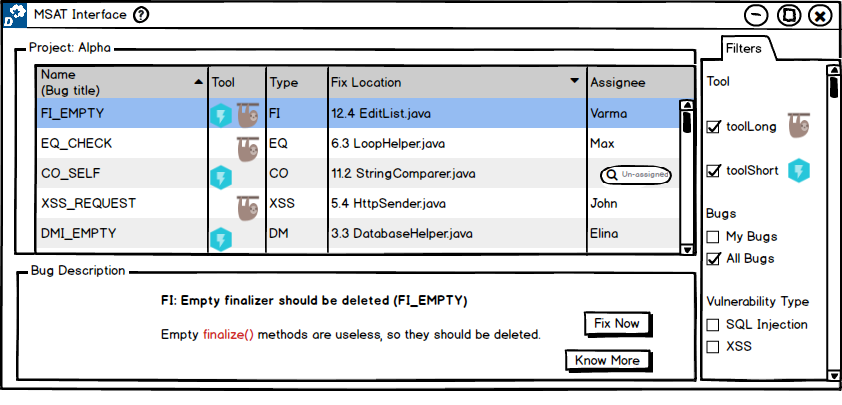
\includegraphics[width=\linewidth]{figures/solution_ideas_snaps/S11_single_list}
	\caption{An interface prototype showing 'single list' solution idea.}
	\label{fig:S11_single_list}
\end{figure}


\textbf{Evaluation}: \\

Quantitative Results: \\

There are five user study participants. Every user has managed to perform all three tasks stated above on the provided prototype representing “single list” solution idea. This evaluation shows that the task success rate is 100 per cent. \\ \\

Among the five users, two users felt this is convenient in considering a final solution idea in showing the analysis results, in comparison to other solution ideas.  In terms of usability on a scale of 0 to 10, where 0 is worst and 10 being the best, five users rated the solution ideas in comparison to alternate solution ideas i.e., separate list and tags as 9,8,8,8,7, which averages to 8. This is highest among the solution ideas. \\ \\

Qualitative Results: \\

Let us now investigate the reasoning behind the user’s choice of solution idea and respective ratings. Users felt the union of bugs from multiple tools is good, and it also gives satisfaction that there are these many bugs in a codebase. Also, easiness in filtering the results and able to go through once getting familiar, easiness in finding a common bug and overall visually appealing. As improvisation for prototype design, one user suggested to add “hide all” button to disable results from all tools and “show all” button for displaying complete results. \\ \\


\textbf{Solution Idea: ( Separate List )} \\

Similar to the previous one, now the idea is showing separate table view for each tool. This idea could be well understood, looking at following \autoref{fig:S11_seperate_list} or a complete prototype images added in appendix. \\ \\


\begin{figure}[hbt!]
	\centering
	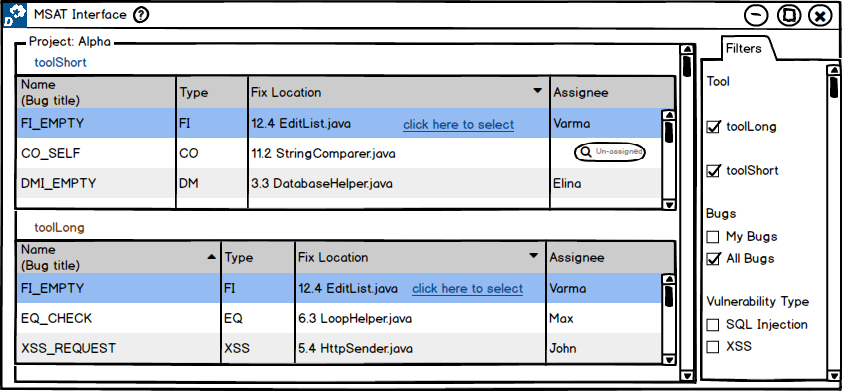
\includegraphics[width=\linewidth]{figures/solution_ideas_snaps/S11_seperate_list}
	\caption{An interface prototype showing 'seperate list' solution idea.}
	\label{fig:S11_seperate_list}
\end{figure}

\textbf{Evaluation}: \\

Quantitative Results: \\

There are five user study participants. Every user has managed to perform all three tasks stated above on the provided prototype representing “single list” solution idea. This evaluation shows that the task success rate is 100 per cent. \\ \\

Among the five users, three users felt this is convenient in considering a final solution idea in showing the analysis results, in comparison to other solution ideas.  In terms of usability on a scale of 0 to 10, where 0 is worst and 10 being the best, five users rated the solution ideas in comparison to alternate solution ideas i.e., single list and tags as 7,8,6,9,8, which averages to 7.6. This is second highest among the three solution ideas. \\ \\


Qualitative Results: \\

Let us now investigate the reasoning behind the user’s choice of solution idea and respective ratings. Users felt the separate lists of bugs from each respective multiple tools is that it is more effective when using more tools, filters do not make sense in this scenario, and there is a suggestion of adding trending, priority as improvisation. Here, trending indicates what the new bug findings and priority indicates the ones which are essential to get fixed. \\ \\

\begin{myboxi}[RQ 1-1: Does a separate list or single list help the user to identify the common bug?]
	Separate list outwins the single list with a slight majority of 3 out 5. 
\end{myboxi}

\clearpage

\textbf{Solution Idea: ( Tags )} \\

As we have seen so far using icons for representing an analysis tool. Now, having a tag name for each tool and used for bug finding results displayed in a complete list view. StackOverflow user interface inspires the present solution idea. This approach could be well understood, looking at following \autoref{fig:S11_tags} or a complete prototype images added in appendix. 
\\

\begin{figure}[hbt!]
	\centering
	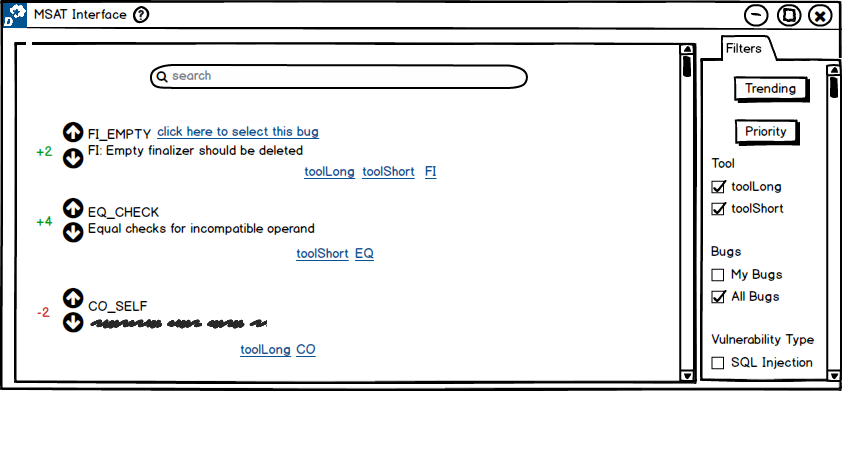
\includegraphics[width=\linewidth]{figures/solution_ideas_snaps/S11_tags}
	\caption{An interface prototype showing 'tags' solution idea.}
	\label{fig:S11_tags}
\end{figure}

\textbf{Evaluation}: \\

Quantitative Results: \\

There are five user study participants. Every user has managed to perform all three tasks stated above on the provided prototype representing “single list” solution idea. This evaluation shows that the task success rate is 100 per cent. \\
Among the five users, no user felt this is convenient in considering a final solution idea in showing the analysis results, in comparison to other solution ideas.  In terms of usability on a scale of 0 to 10, where 0 is worst and 10 being the best, five users rated the solution idea in comparison to alternate solution ideas i.e., single list and separate list as 5,6,4,6,7, which averages to 5.6. This is lowest usability score among the solution ideas. \\

Qualitative Results: \\

Let us now investigate the reasoning behind the user’s choice of solution idea and respective ratings. Users felt the solution idea of using tool names as tags while displaying a complete list of bug findings is that being the user interface a little bit confusing, could not understand how tags work at first impression. They could be habituated once used again and again but confusing at for first time, and the UI is modern but hazy, as a viewer it looks more presentable but being a developer wishes for an easy one and less number of steps. So, overall, even the idea is modern and looks presentable, users did not consider as final choice. \\ \\


\begin{myboxi}[RQ 1-2: Will having tags help in scalability of bugs?]
User felt it does help, but the interface is confusing. Users preferred single list in table format solution idea as it suffices this scalability concern.
\end{myboxi}


\textbf{Solution Idea: ( Summary Screen )} \\

As the standard interface shows a combination of the results from different analysis tools, it is felt ideal for showing a summary of results in the form of graphs. In the present scenario, a solution idea with pie chart with sections resembling the interested grouping/categories found in the usability evaluation report done by Christakis et al. \cite{CB16}. These categories are found out to be the overall sections considered by users going through static analysis results.  This scheme could be well understood, looking at following \autoref{fig:ux1_summary_screen}. \\ \\


\begin{figure}[hbt!]
	\centering
	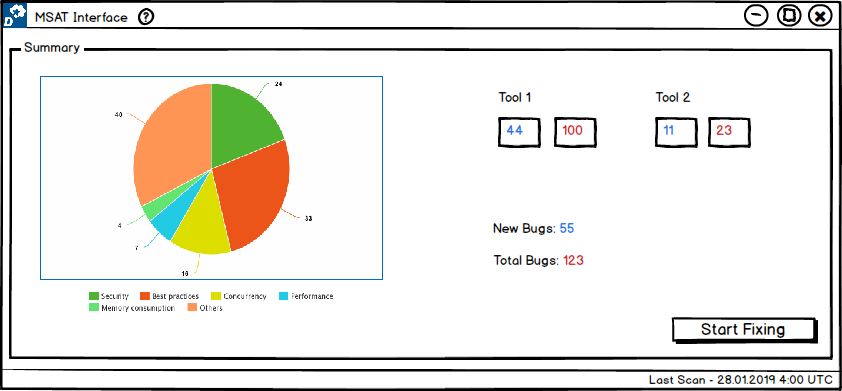
\includegraphics[width=\linewidth]{figures/ux1_summary_screen}
	\caption{An interface prototype showing 'summary screen'.}
	\label{fig:ux1_summary_screen}
\end{figure}

We present the solution idea prototype, then consider the formative feedback. \\

\textbf{Result}: \\

Overall, users have agreed upon its importance in terms of scalability issue. This agreement means there is a need to have such a summary screen which gives an overview of bug findings made by multiple tools and that results in huge numbers in some cases as codebase scales up. \\ \\

Users have recommended having a transition from summary screen to list of bugs as when clicked on particular pi/section in the graph, and then it’s separate list of bugs are shown or at least a separate button named as “view bugs”. One user has suggested to use Line chart as well, which shows the overall performance of an application by having timestamp on X-axis and number of bugs on Y-axis. Also, other user recommends to have a vulnerability scale that determines whether the risk factor is high or low. Also, one user recommended to have a numerical representation. It is about how many bugs got fixed and how many are left. \\ \\

\begin{myboxi}[RQ 1-3: Does the given statistics screen help the user in understanding the analysis results overview? ]
	The statistics screen is conducive, especially when codebase is vast, and we use more analysis tools.
\end{myboxi}
\hfill \break
\subsubsection{RQ 2: What feedback works to know that bug fixing is on-going?}

As part of this primary research question, we are going to evaluate the three feedback mechanisms proposed, i.e., animated icons, progress bar and pending status popup in our designed MSAT-UI ( Multiple Static Analysis Tools – User Interface ). \\

The ‘animated icons’ solution idea demonstrates that when the user chooses a bug finding, and user attempted to fix it by submitting for re-analysis,  respective tool icons with animation like rotating, for example, is shown as feedback for that bug which is under analysis. This idea could be well understood, looking at following \autoref{fig:S12_animated_icons} or a complete prototype images added in appendix. \\

\begin{figure}[hbt!]
	\centering
	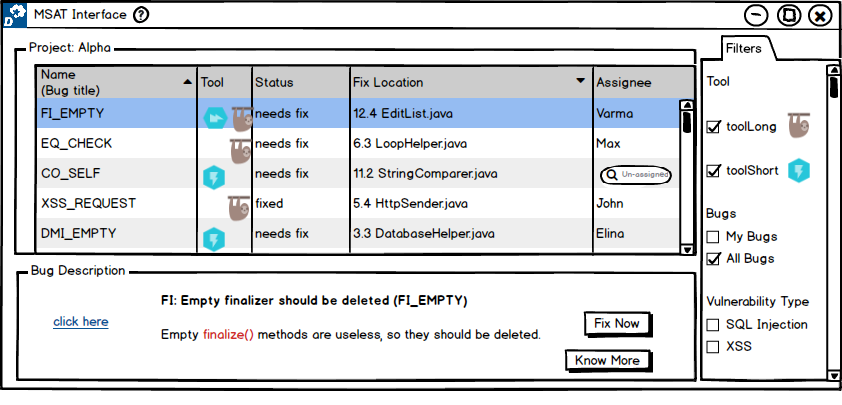
\includegraphics[width=\linewidth]{figures/solution_ideas_snaps/S12_animated_icons}
	\caption{An interface prototype showing 'animated icons'.}
	\label{fig:S12_animated_icons}
\end{figure}

Next, the “progress bar” solution idea is demonstrated as when a user works on a  bug and submitted for analysis.  Then the interface shows progress bars as feedback with how far the tools finishes analysing. It shows progress bars for one or many tools that found that particular bug. This feedback is displayed when clicked on the bug, which is under analysis. Also, the respective icons are shown as blurred, indicating they are under analysis in contrast to previous solution idea. This idea could be well understood, looking at following \autoref{fig:S12_disabled_icons_progress_bar} or a complete prototype images added in appendix. \\ \\


\begin{figure}[hbt!]
	\centering
	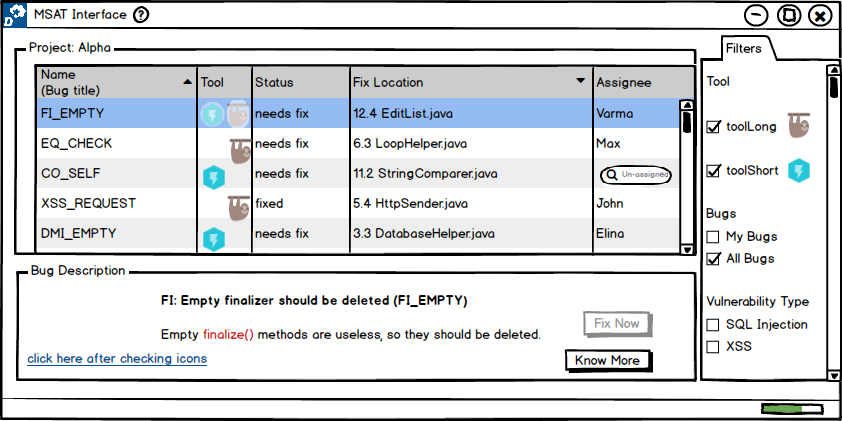
\includegraphics[width=\linewidth]{figures/solution_ideas_snaps/S12_disabled_icons_progress_bar}
	\caption{An interface prototype showing 'progress bar'.}
	\label{fig:S12_disabled_icons_progress_bar}
\end{figure}


Moreover, finally, the third solution idea, i.e., “pending status popup” demonstrates the textual feedback about what the analysis tools are scanning as an example, tool name, timestamp, respective filename with code under analysis. On click of text link named “pending” in the status column in the given table view, it displays the popup. This idea could be well understood, looking at following \autoref{fig:S12_pending_status_popup} or a complete prototype images added in appendix. \\ \\


\begin{figure}[hbt!]
	\centering
	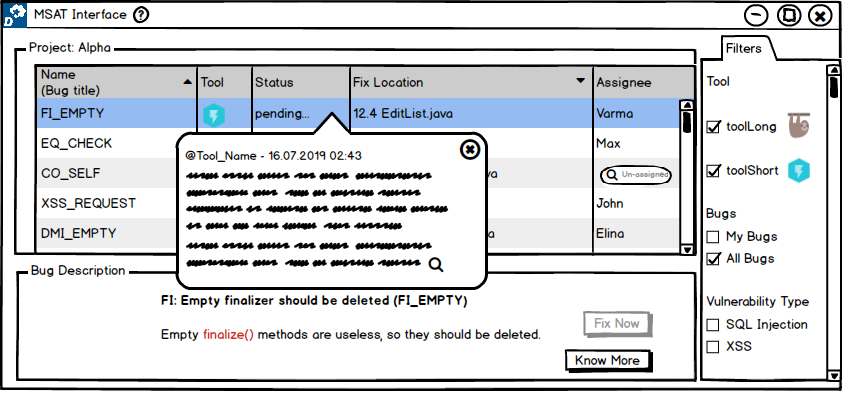
\includegraphics[width=\linewidth]{figures/solution_ideas_snaps/S12_pending_status_popup}
	\caption{An interface prototype showing 'pending status popup'.}
	\label{fig:S12_pending_status_popup}
\end{figure}

The User Scenario, Tasks, and Follow up questionnaire is similar to previous research question. However, the tasks are demonstrated by the designer in order to make the user understands the feedback mechanism ideas. The reason for not doing so is the limitation with prototype builder, i.e., Balsamiq not having dynamic nature in showing animation effects and thereby designer tries to mock the animation effect with multiple clicks which could be tedious if asked the user to do. \\ \\

\textbf{Evaluation}: \\ 

Quantitative Results: \\

Since the designer has performed the tasks, there is no such as task success as seen in previous research question. Among the five users, no user felt any solution idea is not convenient in comparison to other solution ideas to be considered as final solution idea in showing as a feedback during the bug fixing process.  Most users preferred them to have in combinations and especially two users felt progress bar with pending status pop up would be more useful. Nevertheless, users appreciate each feedback in the context of its respective usage scenario. In terms of usability on scale of 0 to 10, where 0 being worst and 10 being the best, 5 users rated “animated icons” solution idea as 7,9,5,8,7 which averages to 7.2, “progress bar” solution idea as 6,9,7,9,9 which averages to 8 and finally “pending status pop up” solution idea as 8,9,8,10,8 which averages to 8.6. \\ \\

Qualitative Results: \\

Let us now investigate the reasoning behind the user’s choice of solution idea and respective ratings. Users felt that any animation would look good, the icons that are disabled in other solution idea, i.e., “progress bar” is confusing. Especially the user with design interests stated that disabled icon could mean they are not clickable as a universal understanding in UI perspective. Users recommended to integrate “status pending popup” idea with others as it is more helpful and informative. \\ \\



\begin{myboxi}[RQ 2-1: Will the animation (rotation) of icons for tools suffice the feedback required by the user? ]
	Animated icons alone does not suffice as feedback. Users interested to see how far the analysis done and also to have more detailed information on it.
\end{myboxi}

\begin{myboxi}[RQ 2-2: Will stating the progress of analysis for each tool be better than animation provided as feedback to the user? ]
	It shows betterment in terms of knowing the progress in completion of analysis.
\end{myboxi}

\begin{myboxi}[RQ 2-3: Does having more textual information with a popup feedback is required by the user? ]
	More information as possible is more beneficial from a user perspective being a developer or tester.
\end{myboxi}

\begin{myboxi}{ \textbf{RQ 2-4: Do users require multiple feedbacks, i.e., any combination of animated icons, progress bar or pending status popup?}} 
\\ \\	Users expressed the opinion of having combination — especially progress bar with pending status popup.
\end{myboxi} 
\hfill \break
Let us switch to the final main question. \\

\subsubsection{RQ 3: How to carry traceability of bug fixing?}

We evaluate the following sub research question in this context. \\

Whether the given UI, i.e., previous commits in the process of fixing a bug-finding with numbers determining the adding or removing of other bugs be able to address the scenario from the user perspective? \\ \\

As part of this primary research question, we evaluate the solution idea of presenting the traceability scenario. TeamScale inspired this solution idea and adapted to our context. This approach could be well understood, looking at following \autoref{fig:S13_revert} or a complete prototype images added in Appendix. In a user study, we explain the concept of traceability to the user, then presents the following User Scenario and a follow-up questionnaire. \\ \\




\begin{figure}[hbt!]
	\centering
	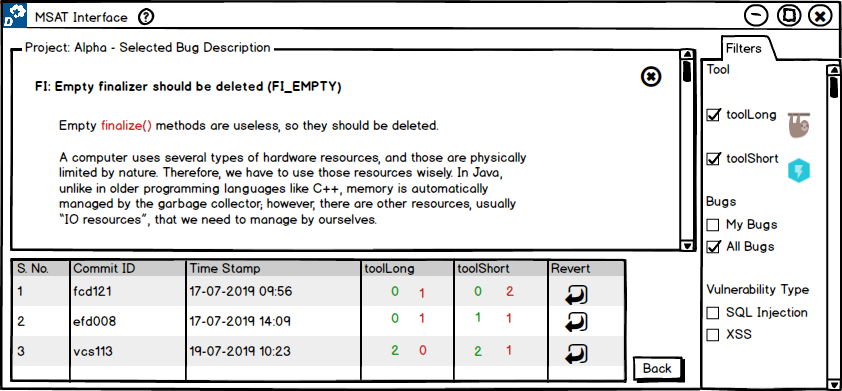
\includegraphics[width=\linewidth]{figures/solution_ideas_snaps/S13_revert}
	\caption{An interface prototype showing 'revert'.}
	\label{fig:S13_revert}
\end{figure}


\textbf{User Scenario}: \\

The user is asked to assume he is working on fixing a bug by doing different commits for every change he did. Bug-finding linked code commits are listed out with numbers indicating the introduction of new bugs and fixing other bugs. This purpose is assumed to help trace the code changes with effect to code quality. Also, there is a revert option to revert the codebase to that instant. \\ \\

\textbf{Follow up}: \\

\begin{enumerate}
\item How the user feel this UI will address the issue?  
\item Is the provide user interface is convenient?
\item How do the user rate in terms of perceived usability ranging from O be lower to 10 be high for provided solution designs in comparison?
\item Do the user imagine anything better UI than this? – Yes/No
\item If it is yes, what does it look like in design?
\end{enumerate}

\textbf{Evaluation}: \\

Quantitative Results: \\

All the participants of user study has agreed upon the presented user interface address the scenario we are looking into and also it is convenient enough. Now, in terms of perceived usability, they have rated as 7,7,8,8 and 7, which averages to 7.4. The rating also shows that prototype is usable enough. \\ \\


Qualitative Results: \\

Let us now investigate the reasoning behind the user’s choice of solution idea and respective ratings. Users felt, in general, it is a good idea for tracing and also interface is excellent. The scenario being relatively new to users and also the proposed design is novel, users have suggested some improvements.  The suggestions are such as a tooltip which explains what green and red values mean and description of bugs, a new column which shows total bugs introduced reported by all tools in combination which will be helpful in easy decision making about revert. \\ \\

\begin{myboxi}{\textbf{RQ 3-1: Whether the given UI, i.e., previous commits in the process of fixing a bug-finding with numbers determining the adding or removing of other bugs be able to address the scenario from the user perspective?}}
\\ \\ The proposed design is helpful for the given scenario.
\end{myboxi}


\subsubsection{Post-test questionnaire}

Do the user think onboard phase, i.e., explain each screen when the user starts up the UI will help the user better understand the UI? - Is it helpful/distractive in this scenario? \\ \\

Evaluation Result: \\

Users felt instead of welcome screens, enough text on user interface would suffice. There is a general recommendation with having an ‘i’ kind of icon which on hover pops up with information saying about what the particular GUI element mean. \\ \\

\begin{myboxi}[Does onboard phase is required to understand the UI better?]
	Enough text on screen would suffice.
\end{myboxi}
\hfill \break
\textbf{Miscellaneous - Users recommendations}: \\

In addition to scenarios considered so far with some suggestions as scope of improvement. Few others could be looked into as well, such as users suggests drop-down option for filters, collapse option would scale better in UI when integrating more tools. Next, some developers might want to see the bugs with different status such as fixed, pending, not fixed. Further, having a search for tool selection instead of long filter list will be more user-friendly. Also, consider renaming “Fix Now” to “Submit” that prototypes show. Next, consider to add “stop analysis”, add a “select” and “deselect all” option for tools in filter list. Also, the user said that it is not useful in having a bug description again while on the code editor screen. Next, the colours used in the design should be standard. Some technical feedback and suggestions from users are that they felt struggle usually in configuring multiple tools. So every tool should come up with easy installation process integrated with IDE. One user recommends to go with 2 or 3 tools in general, and the selection of tools should be done prior and integrate with IDE.

\section{Summary}

During the UX cycle 1, there are five users participated. The evaluation summarises answers for sub research questions as follows. For first primary research question regarding display of results, to answer does a separate list or single list help the user to identify the common bug, we observe that three users chosen separate list solution idea. It is interesting by their choice as its usability score is 7.6 but for single list is 8. Next, having tags does help in scalability, but the interface seems confusing, and so users felt instead to have single list in table format which suffices the scalability issue. Users felt the need of summary screen for analysis results shown with statistics, as tools increases the scalability issue and the understanding of results. Next, about having a statistics screen overview, users have accepted upon its significance in terms of scalability concern. \\ \\
   
For the second primary research question, feedback, while bug fixing is on-going, to answer, will the animation (rotation) of icons for tools suffice the feedback required by the user. Yes! It does and appreciated in the context of its usage scenario. Next, to answer about will stating the progress of analysis for each tool be better than animation provided as feedback to the user, the evaluation shows that users, in fact, like the progress bar feature.  They considered as an added advantage on top of having animation icons in knowing how extent the tool analysis an own bug. Next to answer, does having more textual information as a popup feedback is required by the user, it is found out to be useful for having more information needed by the developer. Finally, to last sub research question, i.e., Do users require multiple feedbacks, i.e., any combination of animated icons, progress bar or pending status popup? Users felt the need for combination as each one plays its significance. \\ \\

Now with third primary research question, traceability of bug fixing, it is observed that users do like the provided user interface design. They felt it is helpful for the given scenario of having previous commits in the process of fixing a bug-finding with numbers determining the adding or removing of other bugs. Finally, to the last sub research of this user experience cycle, i.e., does onboard phase is required to understand the UI better? Evaluation shows that users prefer having enough text on screen would suffice. \\ \\

\section{Lessons Learnt}

The lessons learnt during this first UX design cycle are the following. \\

\begin{enumerate}
\item Having limited mockup screens sometimes surprises when interface does not respond while clicking on some other GUI elements such as buttons or other links on interface which are out of context from a designer perspective.
\item The other lesson that comes with chosen prototype tool builder, i.e., Balsamiq is that when user clicked on keyboard input or with random mouse clicks, results in jumping of mockup screens.  \\ \\
\end{enumerate}

As a workaround to overcome these limitations, we planned to have more mockups although unrelated to the best coverage of possible links on user interface. Next, random jumping of screens with user's keyboard clicks or random mouse clicks is addressed by having control on mouse clicks when possible and by slowing down the process with understanding of users thought process. \\ \\

Also, during this UX design cycle, we have looked at some scenarios. Users have shown their preferences. However, it would be exciting to see whether the choices still hold with new users when a huge code base with more number of bug findings and also when the same codebase integrated with more tools. We have only looked so far at solution ideas for analysis view, so for the next iteration, we are going to look at code view scenarios and their solution ideas.

\let\cleardoublepage\clearpage
